\chapter{Vehicle modelling and parameterisation}\label{cha:Vehicle}

\section{Vehicle modelling}

% Power
\subsection{Power}

modelled power as one of the states
battery capacity from \cite{Falke2004}
integrate power used over the transfer (active thruster * dt * dL/dt * dLn/dL)
panel efficiency from FLP @ Uryu
Power generated
\begin{gather}
P = E_{density} \times\eta_{panel}\times\eta_{area}\times\eta_{converter}\times\cos\theta_{sun} - P_{instruments} - P_{comms}
\end{gather}
sun angle = angle between sun vector and control vector
\begin{gather}
a\cdot b = |a|.|b|\cos{\theta} \\
\theta = \arccos\frac{a\cdot b}{|a|.|b|}
\end{gather}
Batteries 2.8kWh \parencite{Falke2004}
solar panel degradation is directly related to total equivalent \enquote{fluence} (i.e. radiation dose), figure is available
(\cite{Hechler2002} Power degradation modelling in the SMART 1 mission analysis, CNES Seminar on van Allen Radiation Modelization, ESOC/TOS-GMA)
\parencite{Erb_thesis}
10~sqm TEC-STAR GaAs/InP 34 series solar arrays with 200~$\mu$m front cover glass and 500~$\mu$m back cover glass
\begin{equation}
P(t_0) = P_{max} = 1.845\text{kW}
\end{equation}
must integrate the total dosage, where the derivative with respect to time dFdt is approximated as a function of the radius (2.4 per 24 hours - just multiply by deltaT) and initial dosage $\mathfrak{F}$ is zero.
\enquote{state} of fluence can then be looked up on another B-spline (fitted curve) to get relative power degradation, then 
\begin{equation}
P_{actual} = P_{max} \times \mathfrak{R}
\end{equation}
is supplied to the batteries. (need to allow for sun angle too!)
subtract power required for spacecraft bus
graph of unconstrained trajectory power output - explain need for thrust duty cycle parameter $\zeta$

% Propulsion
\subsection{Propulsion}
Arcjet power consumption \& operational Isp, efficiency, thrust based on Birk's work. \autoref{sec:PPT-characteristics}
PPTs similar from Matthias. \autoref{sec:Arcjet-characteristics}
science payload during science phase approx 300~W \parencite{web_BW-1}
\begin{gather}
I_{sp} = \frac{v_e}{g_0} \\
T = I_{sp}.g_0.\dot{m} = v_e.\dot{m} \\
\eta = \frac{T^2}{2\dot{m}P} \\
P = \frac{T^2}{2\dot{m}\eta} 
\end{gather}
modelled around apoapsis for first phase (objective is to raise periapsis outside VABs - apoapsis is already outside)

modelled around periapsis for second phase (objective is to raise orbital energy - Oberth effect means more delta V is gained by burning at low altitude).

optimisable fixed-body thrust vector allows trade-off between thrust angle and solar panel orientation - if the craft isn't thrusting, it can still use the thrust vector controls to point the solar panels at the sun

variable thrust magnitude - arcjet model mass flow rate + power???

PPTs is pulse frequency. Assuming we can run at 3~Hz, maximum thrust is increased.... change whole model?!?

Modelling with initial values of PPT frequency = 1~Hz, computational issues due to transfer being too long. Noticed that the power was a huge surplus, so spoke to the PPT experts (Matthias) who indicated that extra power could be pushed into higher pulse rate on the PPTs, up to 3~Hz. Remodelled based on this (effectively higher thrust and power consumption, but same Isp - this is the principle on which advocates of EP see it as the most efficient feasible propulsion for interplanetary missions).

Due to the particularly non-linear variations with launch date (periodic over 27.5~days based on the Moon's orbit) a good parameterisation of the launch date would be to use two variables, one to increment an integer number of months forwards or backwards, the other a floating point to indicate the number of days either side of the month.

Initially modelled Cruise with 4xPPTs at 1~Hz, took 2298~radians $\Delta$L and about 950~days. Optimisation not possible due to numerical limitations. Modified to 2Hz due to surplus power, simulation took 1347~radians and about 500~days.
\begin{figure}
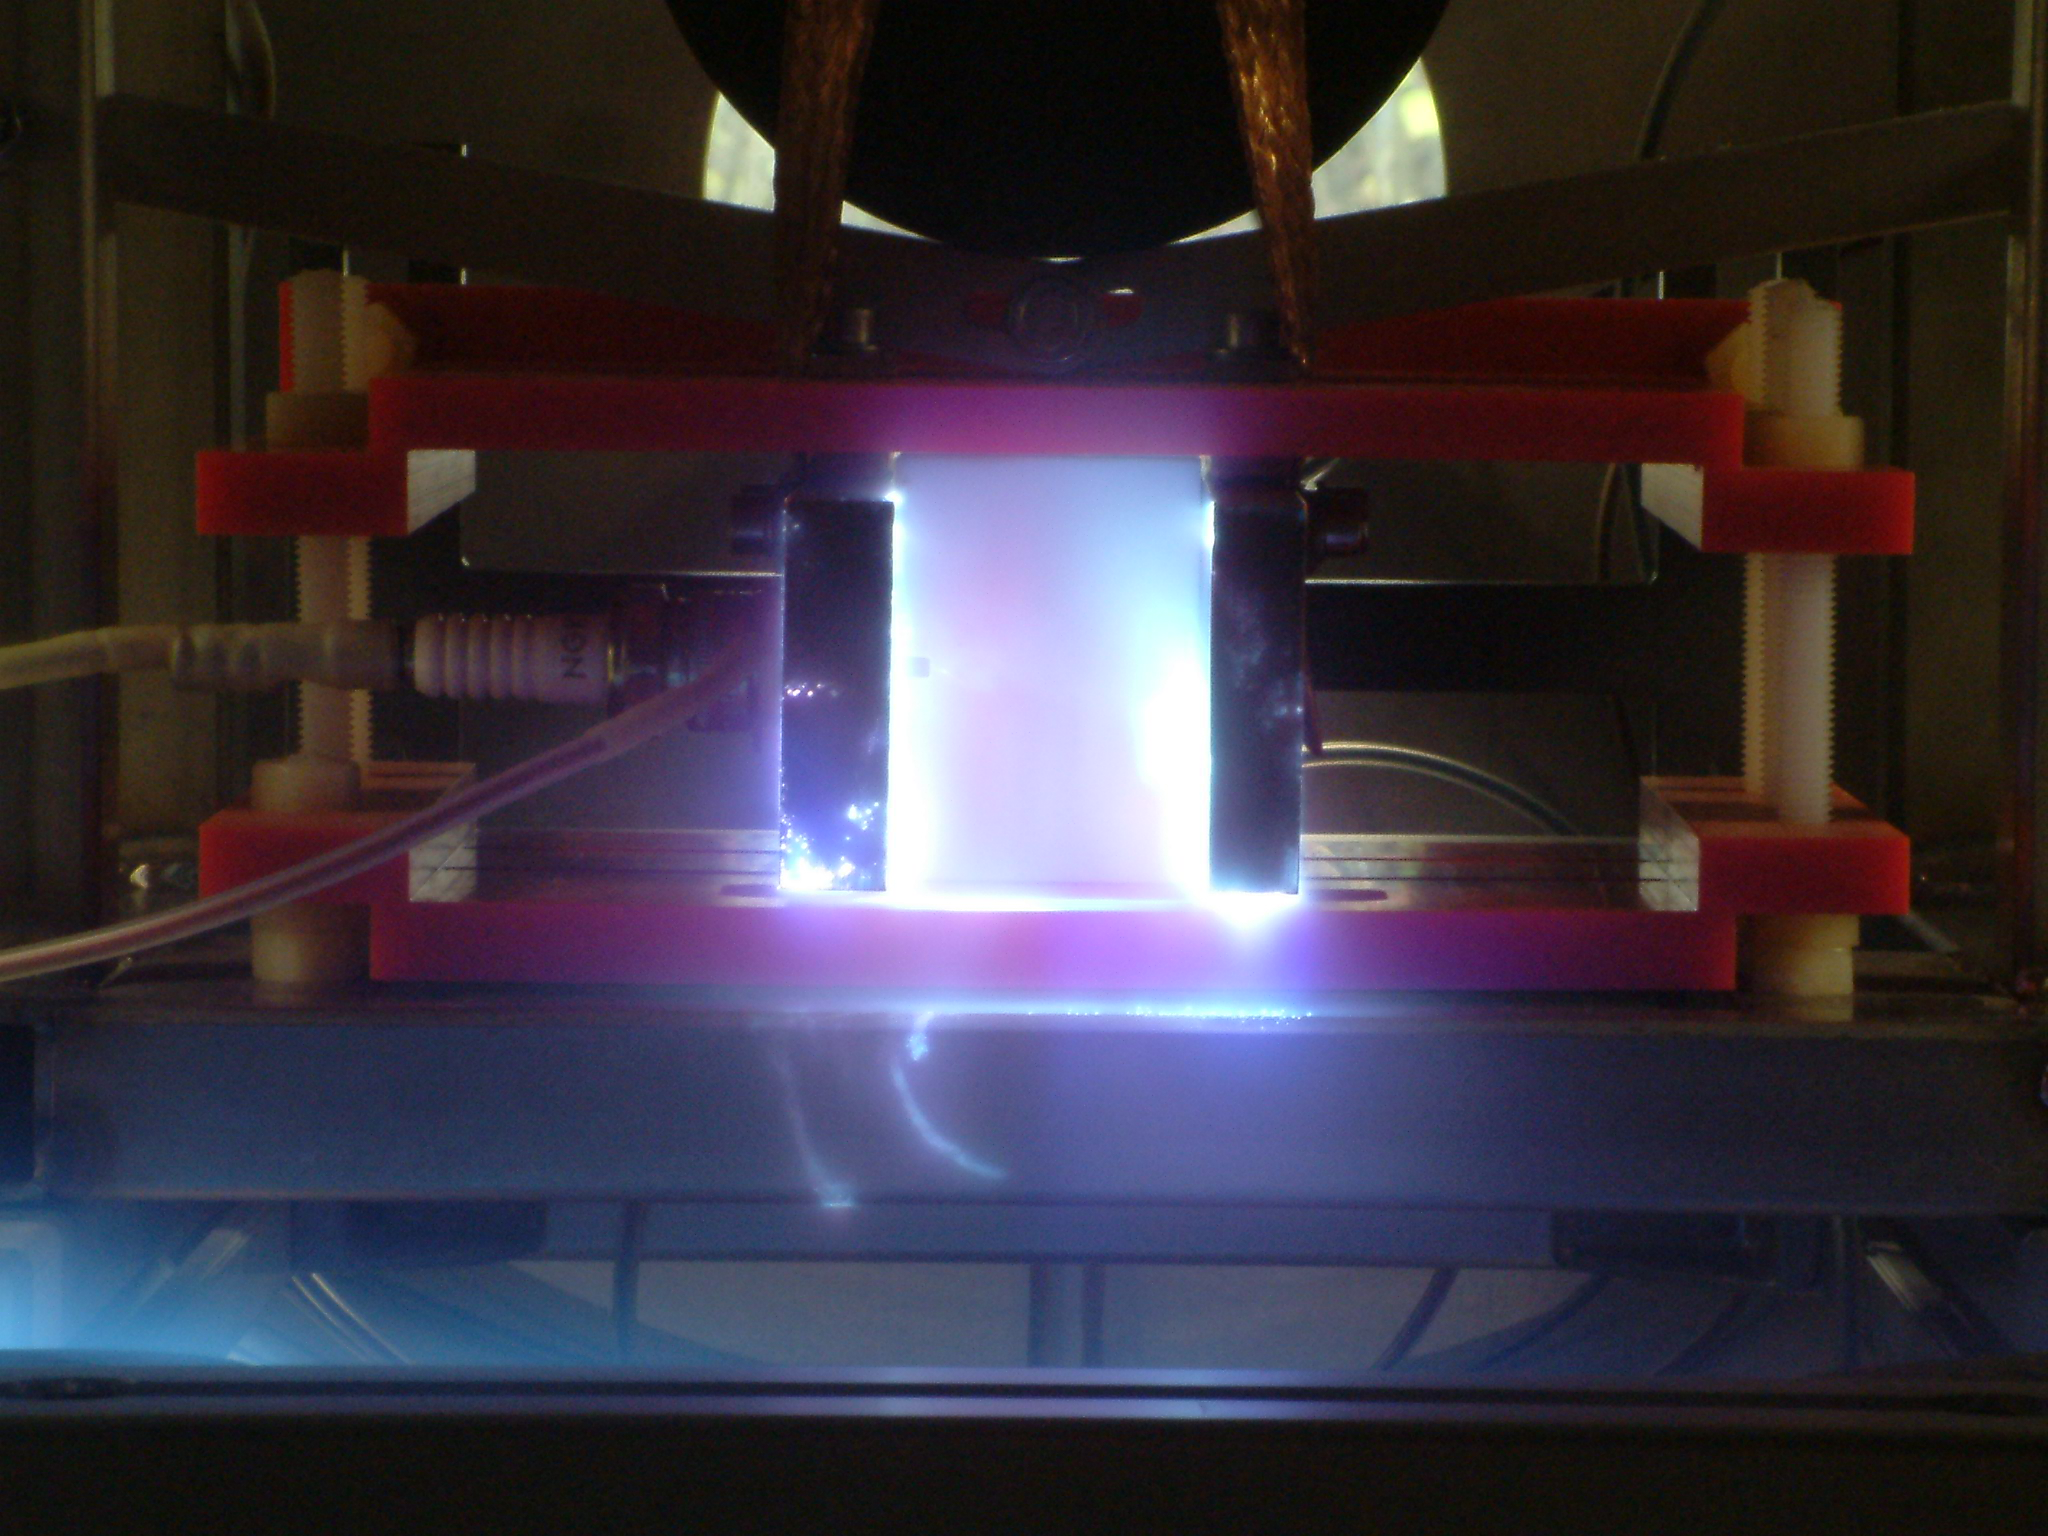
\includegraphics[width=\textwidth]{Images/PPT_test.JPG}
\caption{SIMPLEX PPT during a laboratory test. The spark plug (centre left) ignites an arc between the two electrodes (pointing towards the camera) which vapourises the surface of the block of white PTFE between them. The electric field between the two electrodes then accelerates the plasma towards the camera.}\label{fig:PPT}
\end{figure}
\begin{figure}
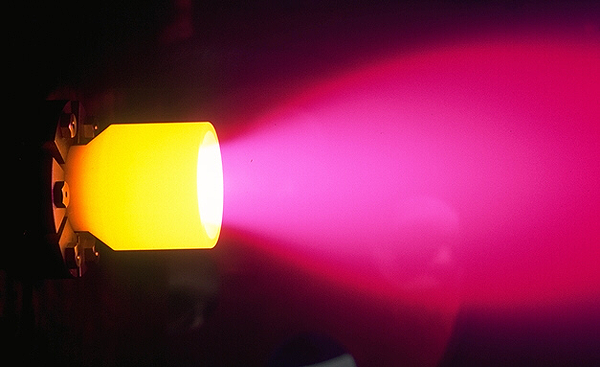
\includegraphics[width=\textwidth]{Images/hiparc_betrieb.png}
\caption{TALOS arcjet during a laboratory test. An arc is generated between the axial cathode and the nozzle anode, which heats up the ammonia, accelerating it outwards.}\label{fig:arcjet}
\end{figure}
Show graphs for low power Cruise phases? 

From the power output, realised that the design could use more power to transfer faster - take many forms. Higher pulse frequency most promising, this linearly increases thrust at exactly the same Isp, at the cost of linearly increasing power consumption. The only limitation is wear and tear to the service life of the thruster; should be proportional to the number of pulses and since each pulse provides a certain Impulse bit, the number of pulses required to perform the lunar transfer should be constant. Thrusters have not been endurance tested yet meaning we don't know how many cycles they can perform. Other constraint is cooling - over about 3~Hz the PTFE is not able to cool properly between cycles and can interfere in the thruster performance. However, some tests performed in Russia (cite Matthias and/or Pedro here?) have successfully used a design similar to SIMPLEX at 20~Hz.

Thrust and power can also be linearly scaled by simply introducing more PPTs to the structure. This has been championed by the PPT designer, Matthias Lau. This option increases the redundancy of the system (and therefore reliability). However, it also carries the associated cost of extra weight.

Finally, extra power can be discharged into each pulse. This increases the Isp and thrust because the plasma is accelerated faster, but the increase is not proportional to the extra power put into each pulse. Therefore the power efficiency drops. Currently the development of the PPTs is focussed on improving the power efficiency, so the performance at this opposite end of the scale is not well characterised/not well known.

% Ground station
\section{Ground station access}
ground stations in stuttgart, USA, japan and australia give continual access during earth orbit

only downtime is when it's behind the moon

needs to rotate to communicate with ground station!!!

approx 250~W for Ka-band, 10~W for S-band. S-band only works in LEO.

% Earth shadow
\section{Earth shadow}

% Reaction wheel
\section{Reaction wheel desaturation}

% Parameterisation
\section{Parameterisation}

How everything is split up and discretised. Time, phases, gridpoints within phases. 

\subsection{Discretisation}

\subsection{Substitution of parameters}\label{sub:subst-param}

\autoref{sec:state-vector} establishes the state vector $\vec{x}=[p,f,g,h,k,L,m,t,E]$, and provides the differential equations with respect to time. However, as outlined in \autoref{sub:Independent-parameter}, the normalised true anomaly, $Ln$, was the independent parameter. Therefore a subsitution of parameters is required to give derivatives with respect to $Ln$, $\frac{d}{dLn}$. Differentiating \autoref{eq:Ln} gives
\begin{subequations}
\begin{gather}
\frac{dLn}{dt}=\frac{1}{\Delta L}\frac{dL}{dt} \\
\frac{dLn}{dt}\cdot\frac{dt}{dL}=\frac{1}{\Delta L} \\
\frac{dLn}{dL}=\frac{1}{\Delta L} \\
\frac{dL}{dLn}=\Delta L
\end{gather}
\end{subequations}

Using this identity, the state differential equations with respect to normalised longitude may be determined.

\begin{subequations}
\begin{align}
\frac{dp}{dLn}&=\frac{dp}{dt}\cdot\frac{dt}{dLn}\\
&=\frac{dp}{dt}\cdot\frac{dt}{dL}\cdot\frac{dL}{dLn}\\
&=\frac{\dot{p}}{\dot{L}}\Delta L
\end{align}
\end{subequations}

%The differential equations for $f$, $g$, $h$, $k$ and $m$ are modified similarly to $p$. $L$ is simply $\frac{dL}{dLn}$. Substituting the parameters of the remaining differential equations gives:
%\begin{subequations}
%\begin{align}
%\frac{dt}{dLn}&=\frac{dt}{dL}\cdot\frac{dL}{dLn}\\
%&= \frac{1}{\dot L}\cdot\Delta L
%\end{align}
%\end{subequations}
%\begin{subequations}
%\begin{align}
%\frac{dE}{dLn} &= \frac{dE}{dt}\cdot\frac{dt}{dL}\cdot\frac{dL}{dLn} \\
%&= \frac{P}{\dot{L}}\cdot\Delta L 
%\end{align}
%\end{subequations}
The remaining differential equations are modified similarly. The final equations are
\begin{subequations}
\begin{gather}
\frac{dp}{dLn}=\frac{\dot{p}}{\dot{L}}\Delta L \\
\frac{df}{dLn}=\frac{\dot{f}}{\dot{L}}\Delta L \\
\frac{dg}{dLn}=\frac{\dot{g}}{\dot{L}}\Delta L \\
\frac{dh}{dLn}=\frac{\dot{h}}{\dot{L}}\Delta L \\
\frac{dk}{dLn}=\frac{\dot{k}}{\dot{L}}\Delta L \\
\frac{dL}{dLn}=\Delta L \\
\frac{dm}{dLn}=\frac{\dot{m}}{\dot{L}}\Delta L \\
\frac{dt}{dLn}=\frac{1}{\dot{L}}\Delta L \\
\frac{dE}{dLn}=\frac{P}{\dot{L}}\Delta L 
\end{gather}
\end{subequations}
where $\dot{p}$, $\dot{f}$,  $\dot{g}$, $\dot{h}$, $\dot{k}$ and $\dot{L}$ are the original time-domain differential equations provided by \textcite{Walker1985}.

\subsubsection{Delta-v calculation}
The universal definition for delta-v was provided in \autoref{sub:Delta-v}. Unfortunately this definition also depends on time-domain integration. Therefore another substitution of parameters is required.
\begin{subequations}
\begin{align}
\Delta v &= \int^{Ln_f}_{Ln_i}\frac{|T|}{m}\frac{\text{dt}}{\text{dLn}}\text{dLn}\\
&= \int^{1}_{0}\frac{|T|}{m}\frac{\text{dt}}{\text{dL}}\cdot\frac{\text{dL}}{\text{dLn}}\text{dLn}\\
&= \int^{1}_{0}\frac{|T|}{m}\frac{\Delta L}{\dot L}\text{dLn}
\end{align}
\end{subequations}

%\section{Oberth effect}
%Thrust more at periapsis, less at apoapsis. Should become more apparent when thrust is not held to $T_{max}$.


% Lunar capture
Even with capture phases provided by arcjet, there is very little thrust available to perform lunar insertion. When simulating the transfer this problem is compounded by the fact that lunar insertion must be predicted very accurately, as simulating a lunar orbit in an Earth-centred frame, or vice-versa, causes the trajectory to periodically appear to move backwards relative to the central body. In other words, the anomaly decreases, which causes computational errors.

review this: Low Energy Motions in the Earth-Moon System, Chaos, and Weak Capture \parencite{Belbruno2007}

aim for a \emph{weak capture} at the Moon. This is a capture where the Kepler energy with respect to the Moon is non-positive and the motion of the particle with respect to the Moon is unstable. Such captures are generally temporary. Weak capture occurs in a special region in phase space about the Moon called the \emph{weak stability boundary}, WSB, rigorously defined by \textcite{Belbruno2004}

all Belbruno stuff is for impulsive transfers; WSB trajectory to the Moon through deep space.

Hiten probe tested aerobraking and WSB transfers. Also Kordylewski clouds.
% Discretisation
\cite{ASTOS_guide} \enquote{all major grid nodes are also control nodes by definition. When the major grid is too coarse for the controls, pure control nodes can be added.} \enquote{Collocation methods ignore any control refinement points.} \enquote{The constraint grid will be ignored [by] SOCS, since SOCS computes constraint evaluation only at each collocation grid point.}
% Parameterisation
% Vehicle
